\documentclass{beamer}

\usepackage{minted}
\usepackage{pgf}
\usepackage{tikz}
\usepackage[utf8]{inputenc}
\usepackage{mdframed}

\BeforeBeginEnvironment{minted}{\begin{mdframed}}
\AfterEndEnvironment{minted}{\end{mdframed}}

\title{Let The Compiler Help You: How To Make The Most Of Scala's Typesystem}
\author{Markus Hauck (@markus1189)}

\date{Scala.IO 2017}
\subject{Computer Science}
\usetheme{codecentric}

\renewcommand\texttt[1]{\mintinline{scala}/#1/}

\usemintedstyle{fruity}

\usetikzlibrary{arrows,automata}

\begin{document}

{
  \usebackgroundtemplate{
\includegraphics[height=\paperheight]{background.jpg}}
  \frame[plain]{\titlepage}
}

\section{Intro}
\label{sec:intro}

\begin{frame}
  \begin{center}
    \frametitle{One Evening}
    
\includegraphics[width=0.6\textwidth]{../pics/lets-program.png}
  \end{center}
\end{frame}

\begin{frame}[fragile]
  \frametitle{Done!?}
\begin{minted}{bash}
> compile
[success] Total time: 42s, completed Nov 2 14:05:42
> run
...
\end{minted}
\end{frame}

\begin{frame}
  \begin{center}
    
\includegraphics[width=0.6\textwidth]{../pics/unsupported.png}
  \end{center}
\end{frame}

\begin{frame}[fragile]
  \frametitle{Done!?}
\begin{minted}{bash}
> compile
[success] Total time: 42s, completed Nov 2 14:05:42
> run
...
\end{minted}
\end{frame}

\begin{frame}
  \begin{center}
    
\includegraphics[width=0.6\textwidth]{../pics/iae.png}
  \end{center}
\end{frame}

\begin{frame}
  \begin{center}
    
\includegraphics[width=0.6\textwidth]{../pics/told-you.png}
  \end{center}
\end{frame}

\begin{frame}[fragile]
  \frametitle{A Better Way}
\begin{minted}[fontsize=\footnotesize]{bash}
> compile
[info] Compiling 1 Scala source to 
  /home/brain/world-domination/target/scala-2.12/classes ...
[error] ConquerWorld.scala:1337:42: type mismatch;
[error]  found   : Int(-42)
[error]  required: PositiveInt
[error]   requiredAssets(-42)
[error]        ^
[error] one error found
[error] (compile:compileIncremental) Compilation failed
\end{minted}
\end{frame}

\begin{frame}
  \begin{center}
    
\includegraphics[width=0.6\textwidth]{../pics/good-compiler.png}
  \end{center}
\end{frame}

\begin{frame}
  \frametitle{Introduction}
  \begin{itemize}
  \item currently: programming as a fight against the compiler
  \item soon: work \textbf{together} with the compiler
  \item tests: \textbf{evidence} it works
  \item types: \textbf{proof} it works
  \item you need to communicate with the compiler
  \end{itemize}
\end{frame}

\begin{frame}
  \frametitle{The Road Ahead}
  \begin{itemize}
  \item Preparations
  \item Be Honest
  \item Forbid it
  \item No Garbage
  \item Only Valid Ops
  \end{itemize}
\end{frame}

\begin{frame}
  \frametitle{Become Friends}
  \begin{itemize}
  \item by default the compiler is a little shy
  \item but once you get friends, you don't want to go back
  \item first thing: unmute him!
    \begin{itemize}
    \item \texttt{-deprecation}
    \item \texttt{-unchecked}
    \item \texttt{-Xfuture}
    \item \texttt{-Xlint:-unused}
    \item \texttt{-Ywarn-unused:imports,privates,locals}
    \end{itemize}
  \item sometimes false positives, see
    \begin{itemize}
    \item \texttt{scalac -X}
    \item \texttt{scalac -Y}
    \end{itemize}
  \end{itemize}
\end{frame}

\begin{frame}
  \frametitle{Not: Documentation}
  \begin{itemize}
  \item documentation is not for the compiler
  \item it is meant for humans (which are bad at it)
  \item avoid: \textbf{context sensitive} reasoning
  \item think: I \textbf{know} this can't happen
  \item use a language that the compiler understands: types
  \end{itemize}
\end{frame}

\begin{frame}
  \frametitle{Case Study: Vending Machine}
  \begin{columns}
    \begin{column}{0.6\textwidth}
      \begin{itemize}
      \item insert coin (50 cents or 1 euro)
      \item push button for drink
      \item abort the transaction and return money
      \end{itemize}
    \end{column}
    \begin{column}{0.4\textwidth}
      \begin{center}
        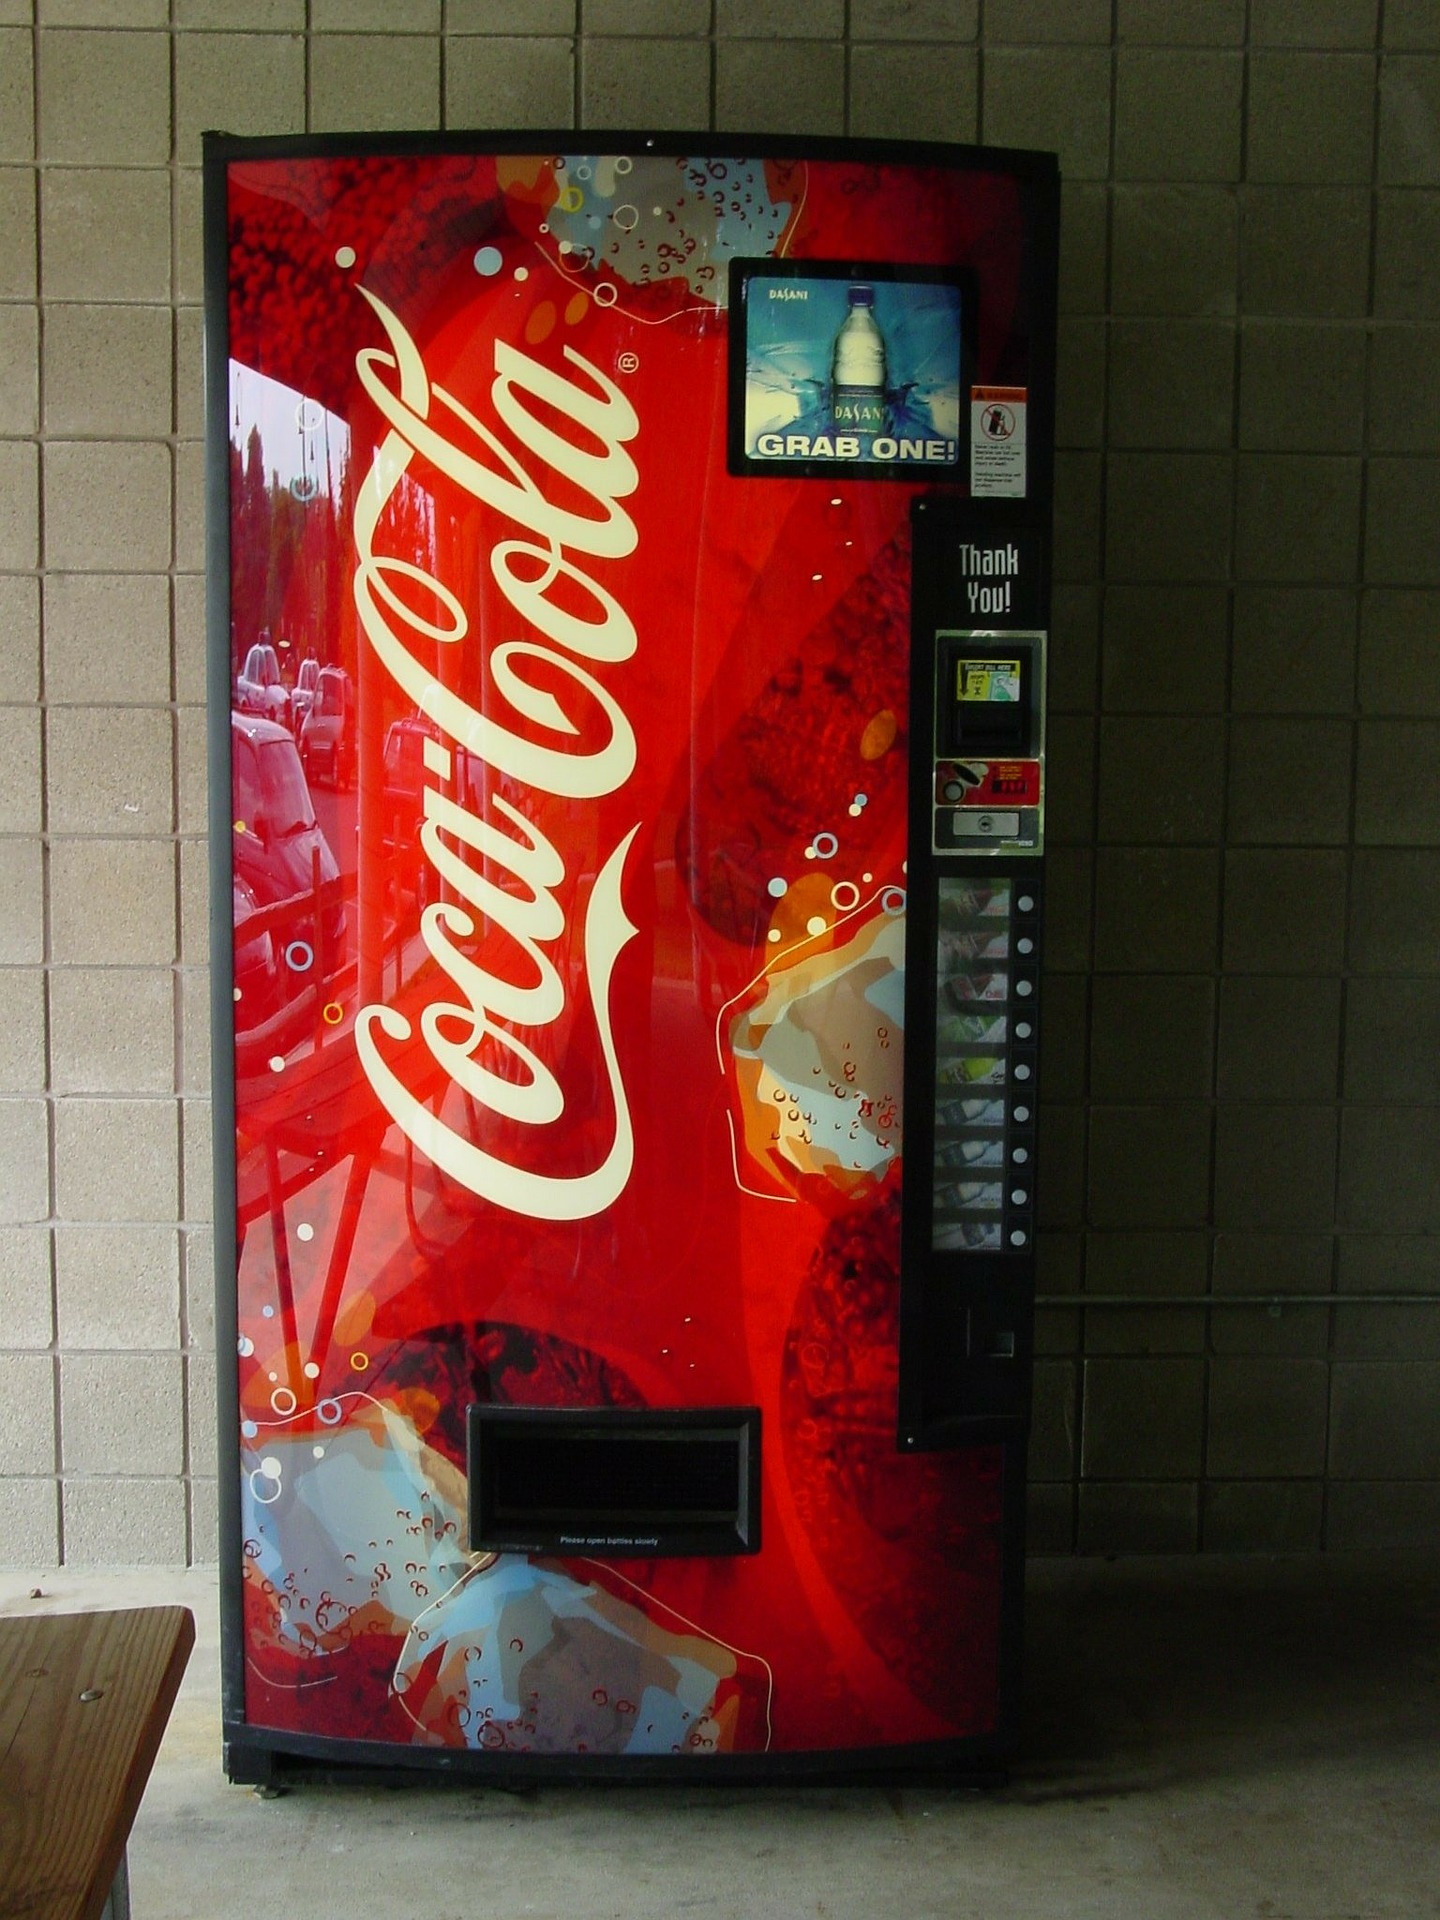
\includegraphics[width=\textwidth]{../pics/vending.jpg}
      \end{center}

    \end{column}
  \end{columns}
\end{frame}

\begin{frame}
  \inputminted[fontsize=\small, firstline=3]{scala}{../src/main/scala/de/codecentric/zero/VendingMachine.scala}
\end{frame}

\begin{frame}
  \frametitle{A First Design}
  \begin{itemize}
  \item what does the compiler know?
  \item what do you as a user of this class know without docs?
  \end{itemize}
  \begin{center}
    
\includegraphics[width=0.5\textwidth]{../pics/docs.jpg}
  \end{center}
\end{frame}

\section{Be Honest}

\begin{frame}
  \frametitle{Step 1: Be Honest}
  \begin{center}
    
\includegraphics[width=\textwidth]{../pics/dog.jpg}
  \end{center}
\end{frame}

\begin{frame}[fragile]
  \frametitle{Get The Max Out Of Your List}
  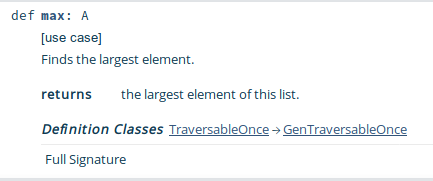
\includegraphics[width=0.8\textwidth]{../pics/list-max.png}
\end{frame}

\begin{frame}[fragile,fragile]
  \frametitle{Get The Max Out Of Your List}
\begin{minted}{scala}
> List[Int](1, 2, 3).max
res0: Int = 3
\end{minted}
\begin{minted}{scala}
> List[Int]().max                                                             
java.lang.UnsupportedOperationException: empty.max                                 
\end{minted}
\end{frame}

\begin{frame}
  \frametitle{Be Honest}
  \begin{itemize}
  \item not honest $\Rightarrow$ no help
  \item \texttt{max} pretends to always return something, which is not
    the case!
  \item tell the compiler this operation can fail
  \item Option: if no result is a result
  \item Either: if there can be errors
  \item Custom ADT:\@if \texttt{Either} doesn't cut it
  \end{itemize}
\end{frame}

\begin{frame}
  \frametitle{Be Honest}
  \begin{itemize}
  \item how does this apply to our case study?
  \item \texttt{insertMoney} can fail
  \item \texttt{pushButton} can fail
  \item \texttt{abort} can fail
  \end{itemize}

  \begin{itemize}
  \item we will fix this later
  \end{itemize}
\end{frame}

\section{Forbid It}

\begin{frame}
  \frametitle{Step 2: If not allowed, forbid it}
  \begin{center}
    
\includegraphics[width=0.5\textwidth]{../pics/forbidden.png}
  \end{center}
\end{frame}

\begin{frame}[fragile,fragile]
  \frametitle{Step 2: If not allowed, forbid it}
  \begin{itemize}
  \item \textbf{every} project has domain classes with invariants
  \item how to verify those invariants?
  \end{itemize}
\begin{minted}{scala}
if (input.isValid) {
  ???
} else {
  throw new Exception("whoopsie")
}
\end{minted}
\begin{minted}{scala}
class ImportantStuff(stuff: Stuff) {
  require(stuff.isImportant, "Not important!")
}
\end{minted}
  \begin{itemize}
  \item but the compiler (and others) does not know this!
  \end{itemize}
\end{frame}

\begin{frame}[fragile]
  \frametitle{If not allowed, forbid it}
\begin{minted}{scala}
case class Email(value: String) extends AnyVal {
  require(isValidEmail(value))
}
\end{minted}
\begin{minted}{scala}
> Email("markus.hauck@codecentric.de")
res1: Email = ...

> Email("Hello World!")
java.lang.IllegalArgumentException: 
  Not a valid email address                      
\end{minted}
\end{frame}

\begin{frame}
  \frametitle{If not allowed, forbid it}
  \begin{itemize}
  \item how can we improve?
  \item for methods, the \textbf{return type} changed
  \item instantiation doesn't have one?
  \item one solution: smart constructors / factories
  \end{itemize}
\end{frame}

\begin{frame}[fragile,fragile]
  \frametitle{If not allowed, forbid it}
\begin{minted}{scala}
abstract case class Email private (...)

object Email {
  def fromString: Either[ValidationError, Email] = 
    ??? // exercise
}
\end{minted}

\begin{minted}{scala}
> Email.fromString("markus.hauck@codecentric.de")
res1: Either[ValidationError, Email] = 
  Right("markus.hauck@codecentric.de")

> Email.fromString("Hello World")
res2: Either[ValidationError, Email] = 
  Left(InvalidEmail)
\end{minted}
\end{frame}

\begin{frame}
  \frametitle{Case Study}
  \begin{itemize}
  \item Okay, back to our case study
  \item we want to fix:
    \begin{itemize}
    \item methods that are not honest
    \item forbid invalid instantiation
    \end{itemize}
  \end{itemize}
\end{frame}

\begin{frame}[fragile,c]
  
  \inputminted[fontsize=\small, firstline=3, lastline=22]{scala}{../src/main/scala/de/codecentric/two/VendingMachine.scala}
\end{frame}

\begin{frame}[fragile,c]
  \inputminted[fontsize=\small, firstline=24, lastline=33]{scala}{../src/main/scala/de/codecentric/two/VendingMachine.scala}
\end{frame}


\begin{frame}
  \frametitle{Case Study: Review}
  \begin{itemize}
  \item we got rid of all exceptions
  \item no way to ``forget'' that something can fail
  \item compiler (coworkers?) now knows quite a bit more
  \item what else can we improve?
  \end{itemize}
\end{frame}

\section{No Garbage}

\begin{frame}
  \frametitle{Step 3: Don't accept garbage}
  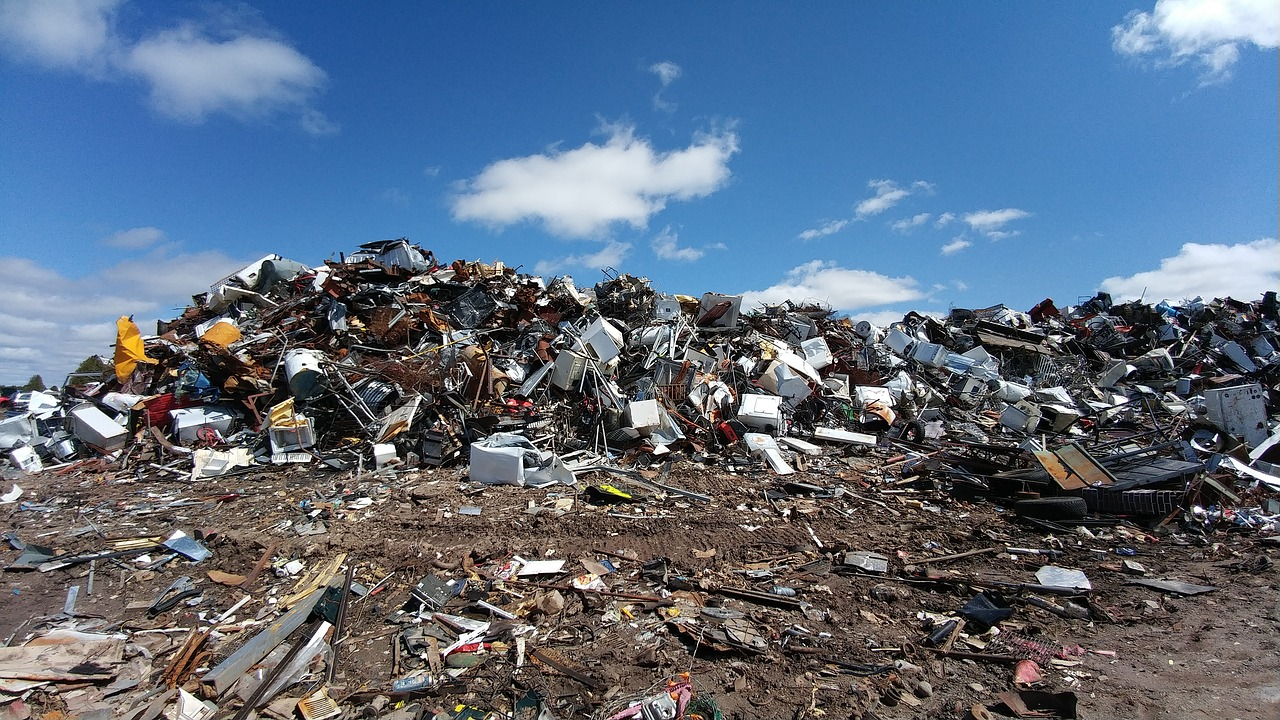
\includegraphics[width=\textwidth]{../pics/scrapyard-2441432_1280.jpg}
\end{frame}

\begin{frame}[fragile,fragile]
  \frametitle{Don't accept garbage input}
  \begin{itemize}
  \item another everyday example:
  \end{itemize}
  \begin{center}
\begin{minted}{scala}
> List(1, 2, 3).take(-42)
\end{minted}
  \end{center}
  \begin{itemize}
  \item Quiz: what happens?
  \end{itemize}
\end{frame}

\begin{frame}[fragile,fragile,fragile]
  \frametitle{Don't accept garbage input}
  \begin{itemize}
  \item another everyday example:
  \end{itemize}
  \begin{center}
\begin{minted}{scala}
> List(1, 2, 3).take(-42)
\end{minted}
  \end{center}
  \begin{itemize}
  \item Quiz: what happens?
  \end{itemize}
\begin{minted}{scala}
res1: List[Int] = List()
\end{minted}
\end{frame}

\begin{frame}
  \frametitle{Don't accept garbage input}
  \begin{itemize}
    
  \item our constructor and methods are quite liberal
  \item they take almost everything!
  \item does the validation really belong in our vending machine?
  \item actually it is the \textbf{caller}'s fault!
  \item better: don't accept garbage and let the caller to the work
  \item push validation to the boundaries of your system
  \item avoid doing it over and over again in program flow
  \end{itemize}
\end{frame}

\begin{frame}[fragile,fragile]
  \frametitle{Putting It Into Practice}
\begin{minted}{scala}
class MailService {
  def sendEmail(mail: String): 
    Either[MailValidationError, MailStatus]
}
\end{minted}

\begin{minted}{scala}
class MailService {
  def sendEmail(mail: Email): MailStatus
}
\end{minted}
\end{frame}

\begin{frame}[fragile]
  \frametitle{Putting It Into Practice}
\begin{minted}{scala}
> List(1, 2, 3).head
res1: Option[Int] = Some(1)
\end{minted}
\begin{minted}{scala}
> NonEmptyList.of(1, 2, 3).head
res1: Int = 1
\end{minted}
\end{frame}

\begin{frame}[fragile,fragile]
  \frametitle{Putting It Into Practice}
\begin{minted}{scala}
sealed abstract class List[+A] {
  def apply(index: Int): A
}
\end{minted}

\begin{minted}{scala}
sealed abstract class List[+A] {
  def apply(index: Natural): A
}
\end{minted}
\end{frame}

\begin{frame}
  \frametitle{How To Validate}
  \begin{itemize}
  \item okay seems like it makes sense to do this
  \item goal: make core logic more focused, factor out error handling
  \item how?
    \begin{itemize}
    \item use a wrapper with smart constructors
    \item use phantom types as ``tags''
    \end{itemize}
  \end{itemize}
\end{frame}

\begin{frame}[fragile,fragile]
  \frametitle{Validation With Smart Constructors}
\begin{minted}{scala}
abstract case class Email private (...)

object Email {
  def fromString: Either[ValidationError, Email] = 
    ??? // exercise
}
\end{minted}
  \begin{itemize}
  \item that works, but becomes cumbersome pretty quick
  \item I \textbf{know} it will succeed!
  \end{itemize}
\begin{minted}{scala}
> Email.fromString("foo@bar.de")
\end{minted}
\end{frame}

\begin{frame}
  \frametitle{Phantom Types}
  \begin{itemize}
  \item phantom type: not associated to any value
  \item only exists at compile time
  \item attach information to values
  \item example: validation of user input
  \item instead of repeated validation ``to be sure'', enforce with types
  \end{itemize}
\end{frame}

\begin{frame}[fragile]
  \frametitle{Phantom Types: The Idea}
  \inputminted[firstline=3]{scala}{../src/main/scala/de/codecentric/UserInput.scala}
\end{frame}

\begin{frame}
  \frametitle{Phantom Types for Tags}
  \begin{itemize}
  \item Creating new classes for invariants works, but very cumbersome
  \item But: Whenever input enters your system: require validation
  \item Avoid validation again and again because of different flows
    through system and refactorings (context-free!)
  \item annoying: static input requires validation
  \item \textit{skipping}: \texttt{Tagged} to avoid wrappers
  \end{itemize}
\end{frame}

\begin{frame}
  \frametitle{Refined}
  \begin{itemize}
  \item the refined library to the rescue
  \item in essence: a \textbf{Refined[T, P]}
  \item actual value \texttt{T} + phantom type for predicate \texttt{P}
  \item no wrapper, no custom phantom type (ADT)
  \item only define your predicate or use the builtin ones
  \item killer feature: perform validation for literals as input at
    compile time
  \end{itemize}
\end{frame}

\begin{frame}[fragile]
  \frametitle{Refined: Predicates}
  \begin{itemize}
  \item DSL to define predicates
  \item many builtins:
    \textcolor{beamer@ccblue}{\href{https://github.com/fthomas/refined\#provided-predicates}{link}}
  \item useful as documentation as well
  \end{itemize}

\begin{minted}{scala}
String Refined Uri
String Refined Uuid
String Refined MatchesRegex[W.`"[0-9]+"`.T]

type ZeroToOne = Not[Less[W.`0.0`.T]] 
  And Not[Greater[W.`1.0`.T]]

type ValidChar = 
  AnyOf[Digit :: Letter :: Whitespace :: HNil]
\end{minted}
  
\end{frame}

\begin{frame}[fragile,fragile]
  \frametitle{Using Refined}
  \inputminted[firstline=8,
  fontsize=\small]{scala}{../src/main/scala/de/codecentric/refined/UserInput.scala}
\begin{minted}[fontsize=\small]{text}
[error] UserInput.scala:15: Predicate failed: (-1 > 0).
[error]   index(List(1, 2, 3))(-1) // compile error
[error]                        ^
[error] one error found
\end{minted}
\end{frame}

\begin{frame}[fragile]
  \frametitle{Refined: Dynamic Input}
  \begin{itemize}
  \item but the macro works only for literal input
  \item dynamic values: you still have to take care
  \end{itemize}
  
\begin{minted}{scala}
> refineV[Positive](fortyTwo)
res1: Either[String, Int Refined Positive] = 
  Right(...)
> refineV[Positive](negativeInt)
res2: Either[String, Int Refined Positive] = 
  Left(...)
\end{minted}
\end{frame}

\begin{frame}
  \frametitle{Case Study}
  \inputminted[fontsize=\small,firstline=8, lastline=22]{scala}{../src/main/scala/de/codecentric/three/VendingMachine.scala}
\end{frame}

\begin{frame}
  \frametitle{Case Study}
  \begin{itemize}
  \item the \texttt{Identifier} is checked by \texttt{refined}
  \item \texttt{insertMoney} only allows valid coins by design
  \item we can get rid of the \texttt{Either} in \texttt{insertMoney}
  \item what else?
  \end{itemize}
\end{frame}

\section{Only Valid Ops}

\begin{frame}
  \frametitle{Step 4: Restrict Valid Operations}
  \begin{center}
    
\includegraphics[width=.8\textwidth]{../pics/control-panel.jpg}
  \end{center}
\end{frame}

\begin{frame}
  \frametitle{Vending State Machine}
  \begin{center}
    \begin{tikzpicture}[->,>=stealth,shorten >=1pt,auto,node
      distance=5cm, semithick]
      \tikzstyle{every
        state}=[fill=beamer@ccblue,draw=none,text=white]

      \node[initial,state] (A) {Idle};
      \node[state] (B) [above right of=A] {Half};
      \node[state] (C) [below right of=B] {Ready};

      \path (A) edge [bend left] node {\textcolor{beamer@ccgreen!130}{50}$\Vert$-} (B) edge node {\textcolor{beamer@ccgreen!130}{1}$\Vert$-} (C) (B)
      edge node {\textcolor{beamer@ccgreen!130}{50}$\Vert$-} (C) edge [bend left, swap] node {\textcolor{beamer@ccgreen!130}{abort}$\Vert$50} (A) (C)
      edge [swap, bend left] node {\textcolor{beamer@ccgreen!130}{abort}$\Vert$1} (A) edge [bend left=50] node
      {\textcolor{beamer@ccgreen!130}{pushButton}$\Vert$drink} (A);
    \end{tikzpicture}
  \end{center}
\end{frame}

\begin{frame}
  \frametitle{Vending State Machine}
  \begin{columns}
    \begin{column}{0.4\textwidth}
      \resizebox{1.2\textwidth}{!}{
        \begin{tikzpicture}[->,>=stealth,shorten >=1pt,auto,node
          distance=3cm, semithick]
          \tikzstyle{every
            state}=[fill=beamer@ccblue,draw=none,text=white]

          \node[initial,state] (A) {Idle};
          \node[state] (B) [above right of=A] {Half};
          \node[state] (C) [below right of=B] {Ready};

          \path (A) edge [bend left] node {\textcolor{beamer@ccgreen!130}{50}$\Vert$-} (B) edge node {\textcolor{beamer@ccgreen!130}{1}$\Vert$-} (C) (B)
          edge node {\textcolor{beamer@ccgreen!130}{50}$\Vert$-} (C) edge [bend left, swap] node {\textcolor{beamer@ccgreen!130}{abort}$\Vert$50} (A) (C)
          edge [swap, bend left] node {\textcolor{beamer@ccgreen!130}{abort}$\Vert$1} (A) edge [bend left=50] node
          {\textcolor{beamer@ccgreen!130}{pushButton}$\Vert$drink} (A);
        \end{tikzpicture}
      }
    \end{column}
    \begin{column}{0.6\textwidth}
      \begin{itemize}
      \item possible:
        \begin{itemize}
        \item 50 $\rightarrow$ 50 $\rightarrow$ pushbutton
        \item 50 $\rightarrow$ abort
        \item 1 $\rightarrow$ pushbutton
        \item 1 $\rightarrow$ abort
        \end{itemize}
      \item available actions depend on the \textbf{implicit state}
      \item methods can return \textbf{different types} depending on the
        state, e.g., abort
      \item so we need to check those two invariants (via types)!
      \end{itemize}
    \end{column}

  \end{columns}
\end{frame}

\begin{frame}[fragile]
  \frametitle{State Machine: States}
  \begin{center}
    \inputminted[fontsize=\small, firstline=3,
    lastline=6]{scala}{../src/main/scala/de/codecentric/four/VendingMachine.scala}
  \end{center}
  \begin{center}
    \resizebox{0.5\textwidth}{!}{
      \begin{tikzpicture}[->,>=stealth,shorten >=1pt,auto,node
        distance=4cm, semithick]
        \tikzstyle{every
          state}=[fill=beamer@ccblue,draw=none,text=white]

        \node[initial,state] (A) {Idle}; \node[state] (B) [above right
        of=A] {Half}; \node[state] (C) [below right of=B] {Ready};

        \path (A) edge [bend left] node
        {\textcolor{beamer@ccgreen!130}{50}$\Vert$-} (B) edge node
        {\textcolor{beamer@ccgreen!130}{1}$\Vert$-} (C) (B) edge node
        {\textcolor{beamer@ccgreen!130}{50}$\Vert$-} (C) edge [bend
        left, swap] node
        {\textcolor{beamer@ccgreen!130}{abort}$\Vert$50} (A) (C) edge
        [swap, bend left] node
        {\textcolor{beamer@ccgreen!130}{abort}$\Vert$1} (A) edge [bend
        left=50] node
        {\textcolor{beamer@ccgreen!130}{pushButton}$\Vert$drink} (A);
      \end{tikzpicture}
    }
  \end{center}

\end{frame}

\begin{frame}[fragile]
  \frametitle{State Machine: Vending Machine}
  \inputminted[firstline=8, lastline=25, fontsize=\small]{scala}{../src/main/scala/de/codecentric/four/VendingMachine.scala}
\end{frame}

\begin{frame}[fragile]
  \frametitle{State Machine: Typeclass}
  \inputminted[firstline=31, lastline=42, fontsize=\small]{scala}{../src/main/scala/de/codecentric/four/VendingMachine.scala}
\end{frame}

\begin{frame}[fragile]
  \frametitle{State Machine: Implicit Evidence}
  \inputminted[firstline=44, lastline=48, fontsize=\small]{scala}{../src/main/scala/de/codecentric/four/VendingMachine.scala}
\begin{center}
    \resizebox{0.5\textwidth}{!}{
      \begin{tikzpicture}[->,>=stealth,shorten >=1pt,auto,node
        distance=4cm, semithick]
        \tikzstyle{every
          state}=[fill=beamer@ccblue,draw=none,text=white]

        \node[initial,state] (A) {Idle}; \node[state] (B) [above right
        of=A] {Half}; \node[state] (C) [below right of=B] {Ready};

        \path (A) edge [bend left] node
        {\textcolor{beamer@ccgreen!130}{50}$\Vert$-} (B) edge node
        {\textcolor{beamer@ccgreen!130}{1}$\Vert$-} (C) (B) edge node
        {\textcolor{beamer@ccgreen!130}{50}$\Vert$-} (C) edge [bend
        left, swap] node
        {\textcolor{beamer@ccgreen!130}{abort}$\Vert$50} (A) (C) edge
        [swap, bend left] node
        {\textcolor{beamer@ccgreen!130}{abort}$\Vert$1} (A) edge [bend
        left=50] node
        {\textcolor{beamer@ccgreen!130}{pushButton}$\Vert$drink} (A);
      \end{tikzpicture}
    }
  \end{center}
\end{frame}

\begin{frame}[fragile]
  \frametitle{State Machine: Implicit Evidence}
  \inputminted[firstline=50, lastline=54, fontsize=\small]{scala}{../src/main/scala/de/codecentric/four/VendingMachine.scala}
\begin{center}
    \resizebox{0.5\textwidth}{!}{
      \begin{tikzpicture}[->,>=stealth,shorten >=1pt,auto,node
        distance=4cm, semithick]
        \tikzstyle{every
          state}=[fill=beamer@ccblue,draw=none,text=white]

        \node[initial,state] (A) {Idle}; \node[state] (B) [above right
        of=A] {Half}; \node[state] (C) [below right of=B] {Ready};

        \path (A) edge [bend left] node
        {\textcolor{beamer@ccgreen!130}{50}$\Vert$-} (B) edge node
        {\textcolor{beamer@ccgreen!130}{1}$\Vert$-} (C) (B) edge node
        {\textcolor{beamer@ccgreen!130}{50}$\Vert$-} (C) edge [bend
        left, swap] node
        {\textcolor{beamer@ccgreen!130}{abort}$\Vert$50} (A) (C) edge
        [swap, bend left] node
        {\textcolor{beamer@ccgreen!130}{abort}$\Vert$1} (A) edge [bend
        left=50] node
        {\textcolor{beamer@ccgreen!130}{pushButton}$\Vert$drink} (A);
      \end{tikzpicture}
    }
  \end{center}
\end{frame}

\begin{frame}
  \frametitle{State Machines: Usage}
  \inputminted[firstline=63]{scala}{../src/main/scala/de/codecentric/four/VendingMachine.scala}
\end{frame}

\begin{frame}
  \frametitle{State Machines: Summary}
  \begin{itemize}
  \item calling methods only compiles when it makes sense
  \item eliminates our \textbf{Either} return types
  \item but: restricted to immutability (change type parameters)
  \item potentially less code than inheritance (and less weird)
  \end{itemize}
\end{frame}

\section{Conclusion}

\begin{frame}
  \begin{center}
    
\includegraphics[width=.55\textwidth]{../pics/meme.jpg}
  \end{center}

\end{frame}

\begin{frame}
  \frametitle{The Compiler Is There To Help!}
  \begin{center}
    
\includegraphics[width=0.75\textwidth]{../pics/robot.jpg}
  \end{center}
  \vfill
  \begin{center}
    {\Huge THANKS!}
    \href{https://github.com/markus1189/scala-io-compiler-help}{https://github.com/markus1189/scala-io-compiler-help}
  \end{center}
\end{frame}

\begin{frame}[fragile]
  \frametitle{Bonus: Exercise}
  \begin{itemize}
  \item our vending machine is still quite liberal
  \end{itemize}

\begin{minted}{scala}
val machine: VendingMachine[Ready] = 
  VendingMachine.initial.insertEuro()

val drink1 = machine.pushButton()._2
val drink2 = machine.pushButton()._2
// ...
\end{minted}
    \begin{itemize}
    \item how could we restrict this \textbf{with types}?
    \item hint: limit access to the state machine
  \end{itemize}
\end{frame}

\end{document}
